%\document{article}
\documentclass[UTF8]{ctexart}
\usepackage{listings} 
\usepackage{amsmath}
\usepackage{graphicx}
\usepackage{fancyhdr}
\usepackage{float}


\title{寄存器文件}
\author{PB16030899 朱河勤}
\pagestyle{fancy}
\lhead{PB16030899 朱河勤}
\chead{寄存器文件}
\rhead{2018/4/5}
\begin{document}
\maketitle
\tableofcontents

\section{实验目的}

\paragraph{1}熟练掌握时序逻辑电路的设计方法
\paragraph{2}训练综合各个模块的能力


\section{实验平台}
gtkwave+iverilog


\section{实验原理}
\begin{figure}[H]
  \centering
  \includegraphics[width=1\textwidth]{../../../tmp/prin.png}
\end{figure}


\section{实验要求}
\subsection{总体要求}
设计一64*32bit的寄存器文件,即64个32位的寄存器文件(寄存器组)
具备一组读端口及一组写端口
\paragraph{*}具备一组读端口及一组写端口
\paragraph{*}通过读端口可从0~31号的任意地址读取数据
\paragraph{*}通过写端口可向0~31号的任意地址写入数据
\paragraph{*}通过读端口可从0~31号的任意地址读取数据
\subsection{寄存器文件要求}
设计一64*32bit的寄存器文件,即64个32位的寄存器文件(寄存器组)
具备一组读端口及一组写端口
\paragraph{*}读端口可从0~31号的任意地址读取数据
\paragraph{*}写端口可向0~31号的任意地址写入数据
\paragraph{*}复位值可自行指定

\subsection{功能要求}
\paragraph{1}调用实验一ALU,完成以下功能
寄存器文件组r0,r1初始化为2,2,其他所有寄存器初始化为0
在clk控制下,依次完成以下计算,注意每个clk至多允许完成一次计算
r0+r1->r2
r1+r2->r3
r2+r3->r4
……
r61+r62->r63
\paragraph{2}结果在仿真中显示

\section{实验分析}
\paragraph{1}设计regfile, 读写端口各一个,考虑当读写地址一样时的解决方案
\paragraph{2}设计alu,实现加法
\paragraph{3}设计控制模块,实现地址的选择
\paragraph{4}设计top模块,注意在一个时钟周期中实现求和,变量值的变化达到求斐波那契数列
\section{实验结果}

\begin{figure}[H]
  \centering
  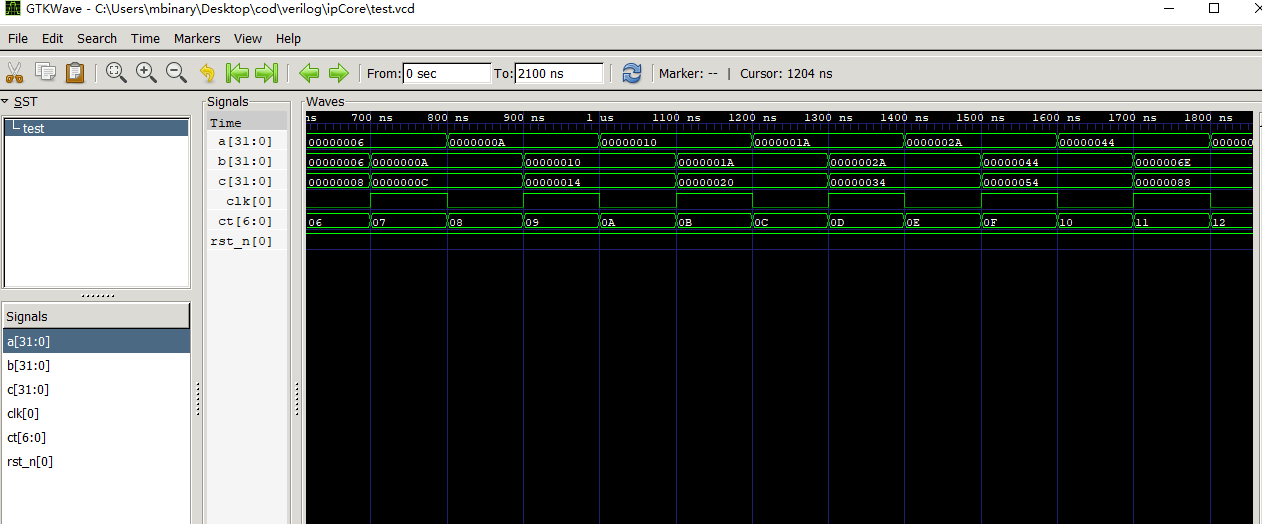
\includegraphics[width=1\textwidth]{reg.png}
\end{figure}



\section{源代码}

\begin{lstlisting}[language=verilog],




module alu(
        input signed  [31:0] alu_a,
		input signed  [31:0] alu_b,
		input 		  [4:0] alu_op,
		output 		  [31:0] alu_out);
		
		reg [31:0] res;
		assign alu_out = res;
		
		always@(*)
		begin
			case(alu_op)
			0:res=0;
			1:res=alu_a+alu_b;
			2:res=alu_a-alu_b;
			3:res=alu_a&alu_b;
			4:res=alu_a|alu_b;
			5:res=alu_a ^ alu_b;
			6:res= ~(alu_a|alu_b);

			endcase
		end
endmodule


module control(
    input clk,rst_n,
    output wEna,
    output [5:0] r1,w
    );
    reg  [5:0] ct =1;
    
    assign wEna = 1;
    assign  r1 = ct,
			w = ct+1;
    
    always@(posedge clk,negedge rst_n)
        begin
            if(~rst_n || ct==63) ct=1;
            else ct =ct+1;
        end
endmodulemodule regfile(
    input           clk,
    input           rst_n,
    input	[5:0]	rAddr1,
    output  [31:0]	rDout1,
    input	[5:0]	wAddr,
    input	[31:0]  wDin,
    input			wEna
);

reg [31:0]  data  [0:63];
reg [31:0] tmp ;

initial begin
data[0] = 2 ;
data[1] = 2 ;
data[2] = 0 ;
data[3] = 0 ;
data[4] = 0 ;
data[5] = 0 ;
data[6] = 0 ;
data[7] = 0 ;
data[8] = 0 ;
data[9] = 0 ;
data[10] = 0 ;
data[11] = 0 ;
data[12] = 0 ;
data[13] = 0 ;
data[14] = 0 ;
data[15] = 0 ;
data[16] = 0 ;
data[17] = 0 ;
data[18] = 0 ;
data[19] = 0 ;
data[20] = 0 ;
data[21] = 0 ;
data[22] = 0 ;
data[23] = 0 ;
data[24] = 0 ;
data[25] = 0 ;
data[26] = 0 ;
data[27] = 0 ;
data[28] = 0 ;
data[29] = 0 ;
data[30] = 0 ;
data[31] = 0 ;
data[32] = 0 ;
data[33] = 0 ;
data[34] = 0 ;
data[35] = 0 ;
data[36] = 0 ;
data[37] = 0 ;
data[38] = 0 ;
data[39] = 0 ;
data[40] = 0 ;
data[41] = 0 ;
data[42] = 0 ;
data[43] = 0 ;
data[44] = 0 ;
data[45] = 0 ;
data[46] = 0 ;
data[47] = 0 ;
data[48] = 0 ;
data[49] = 0 ;
data[50] = 0 ;
data[51] = 0 ;
data[52] = 0 ;
data[53] = 0 ;
data[54] = 0 ;
data[55] = 0 ;
data[56] = 0 ;
data[57] = 0 ;
data[58] = 0 ;
data[59] = 0 ;
data[60] = 0 ;
data[61] = 0 ;
data[62] = 0 ;
data[63] = 0 ;
end

assign rDout1 = tmp;

always@(*)
    if(rAddr1 == wAddr && wEna) tmp  = wDin;
    else tmp = data[rAddr1];
    
always@(posedge clk , negedge rst_n)
    begin
        if(~rst_n ) begin
        data[0] = 2 ;
        data[1] = 2 ;
        data[2] = 0 ;
        data[3] = 0 ;
        data[4] = 0 ;
        data[5] = 0 ;
        data[6] = 0 ;
        data[7] = 0 ;
        data[8] = 0 ;
        data[9] = 0 ;
        data[10] = 0 ;
        data[11] = 0 ;
        data[12] = 0 ;
        data[13] = 0 ;
        data[14] = 0 ;
        data[15] = 0 ;
        data[16] = 0 ;
        data[17] = 0 ;
        data[18] = 0 ;
        data[19] = 0 ;
        data[20] = 0 ;
        data[21] = 0 ;
        data[22] = 0 ;
        data[23] = 0 ;
        data[24] = 0 ;
        data[25] = 0 ;
        data[26] = 0 ;
        data[27] = 0 ;
        data[28] = 0 ;
        data[29] = 0 ;
        data[30] = 0 ;
        data[31] = 0 ;
        data[32] = 0 ;
        data[33] = 0 ;
        data[34] = 0 ;
        data[35] = 0 ;
        data[36] = 0 ;
        data[37] = 0 ;
        data[38] = 0 ;
        data[39] = 0 ;
        data[40] = 0 ;
        data[41] = 0 ;
        data[42] = 0 ;
        data[43] = 0 ;
        data[44] = 0 ;
        data[45] = 0 ;
        data[46] = 0 ;
        data[47] = 0 ;
        data[48] = 0 ;
        data[49] = 0 ;
        data[50] = 0 ;
        data[51] = 0 ;
        data[52] = 0 ;
        data[53] = 0 ;
        data[54] = 0 ;
        data[55] = 0 ;
        data[56] = 0 ;
        data[57] = 0 ;
        data[58] = 0 ;
        data[59] = 0 ;
        data[60] = 0 ;
        data[61] = 0 ;
        data[62] = 0 ;
        data[63] = 0 ;
        end
        else
            data[wAddr] = wEna ? wDin: data[wAddr];
end

endmodule
`timescale 1ns / 1ps


`timescale 1ns / 1ps


module test();

initial begin 
	$dumpfile("test.vcd");
	$dumpvars(1,test);
	end

 reg clk=0;
 reg [6:0] ct=0;
   reg rst_n = 1;
   wire [31:0] a,b,c;
    top top(clk,rst_n,a,b,c);
always #100 
    begin 
        if(ct==20) $finish;
        else begin 
        ct=ct+1 ;   
        clk=~clk; 
        
        end
    end 
always #200 $display("in sim: %g + %g = %g , At time %t", a,b,c,$time);
endmodule



//top  
`timescale 1ns / 1ps

module top(
    input           clk,
    input           rst_n,
    output  [31:0] oa,ob,oc
);


wire [5:0]	rAddr1, wAddr;
wire [31:0] rdata,w;
reg [31:0] tmp=0,sum = 2;
wire wEna;
reg [31:0] res=2;

control ctrl(clk,rst_n, wEna , rAddr1,wAddr);

regfile  regfile(clk,rst_n,rAddr1,rdata,wAddr,sum,wEna);
alu alu(tmp,rdata,1,w);
assign oa = tmp,
        ob = rdata,
        oc = res;
always @(posedge clk) res = w;
//always @*
//$display("in top: tmp,t,rdata,sum,w,raddr= %g,%g,%g,%g,%g",tmp,t,rdata,sum,w,rAddr1);
always @(negedge clk)
    begin 
        tmp <=rdata;
        sum <= w;
        
    end



endmodule


\end{lstlisting}

\end{document}